\section{Universality \& Completeness}

As stated in \cite{duncan2020simplification}, the ZX-Calculus is (approximately) universal because any linear map can be represented as a ZX-diagram. Therefore, any valid quantum circuit can be described as a ZX diagram. Additionally, it can be shown that ZX-Calculus is complete for circuits that are expressed using the \textit{Clifford+T} gates. This means that any two circuits in this family can be transformed into each other by a series of rewrite rules from above.
In particular, this means that if a simplified version of the circuit exists, it can be found by the rules of the ZX-Calculus.
Figure \ref{fig:simplification-idea} shows an example of such a simplification process.

\begin{figure}[h!]
    \centering
    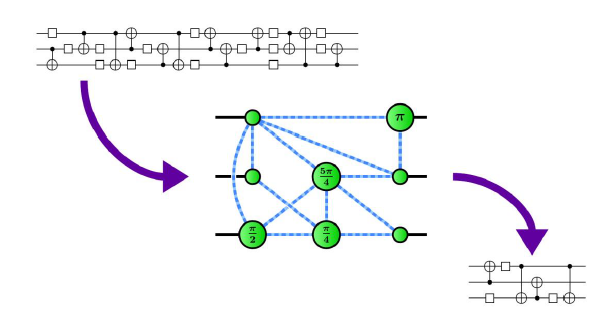
\includegraphics[width=0.4\textwidth]{images/simplification-idea.png}
    \caption{Simplification process\cite{duncan2020simplification-image}}
    \label{fig:simplification-idea}
\end{figure}